\subsection{Menü}



\subsubsection{MenuDataStructures}
Dieses Paket stellt Datenstrukturen für das Menü bereit. 
Unter anderem existiert eine Klasse MiniMapPosition, die 
die Koordinaten des Spielers auf der MiniMap speichert, 
und die Klasse SeedEntry, die zur Speicherung von Seeds 
verwendet wird. Seeds werden jedoch nicht hier gespeichert, 
sondern in einer .properties Datei die in SeedConfig
verwaltet wird.
\par

\begin{figure}[!h]
    \centering
    \centering
        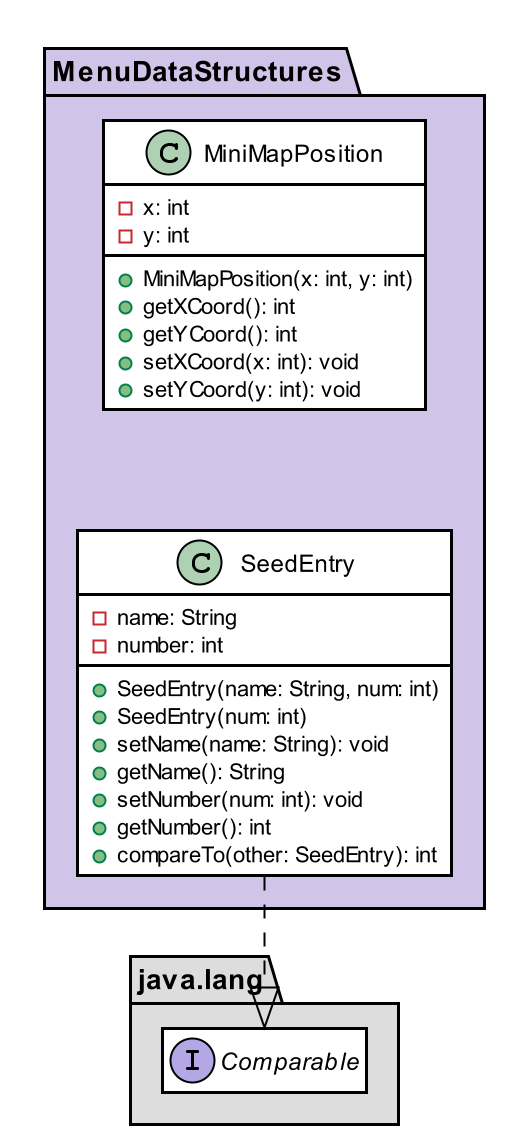
\includegraphics[width=.45\linewidth]{./GUI/GUI_Bilder/MenuDataStructures.png}
          \caption{Paket MenuDataStructures}
           \label{fig:MenuDataStructures}
\end{figure}
    \pagebreak
    \paragraph{\underline{MiniMapPosition}}\label{mmp} \mbox{}\\
        Diese Klasse stellt eine Datenstruktur für die 
        Positionen eines Spielers auf der MiniMap bereit.
        Sie besitzt eine X- und Y-Koordinate, sowie Getter
        und Setter.\\
        \par
        \textbf{Attribute}
        \begin{itemize}
            \item \textit{- int x}  
                \begin{leftbar}[0.9\linewidth]
                    Enthält die X-Koordinate eines Spielers auf 
                    der MiniMap.
                \end{leftbar}
            \item \textit{- int y} 
                \begin{leftbar}[0.9\linewidth]
                    Enthält die Y-Koordinate eines Spielers auf 
                    der MiniMap.
                \end{leftbar}
        \end{itemize}
        \textbf{Methoden}					
        \begin{itemize}
            \item \textit{+ MiniMapPosition(int x, int y)}
                \begin{leftbar}[0.9\linewidth]
                    Dieser Konstruktor speichert den übergebenen Namen und die 
                    Ziffernreihenfolge des neu erstellten Seed-Eintrag Objektes.\\
                    \textbf{@param x} Die zu setzende X-Koordinate.\\
                    \textbf{@param y} Die zu setzende Y-Koordinate.
                \end{leftbar}
            \item \textit{+ getXCoord(): int}
                \begin{leftbar}[0.9\linewidth]
                    Getter für die X-Koordinate eines Spielers auf 
                    der MiniMap.\\
                    \textbf{@return} Die X-Koordinate.
                \end{leftbar}
            \item \textit{+ getYCoord(): int}
                \begin{leftbar}[0.9\linewidth]
                    Getter für die Y-Koordinate eines Spielers auf 
                    der MiniMap.\\
                    \textbf{@return} Die Y-Koordinate.
                \end{leftbar}
            \item \textit{+ setXCoord(int x): void}
                \begin{leftbar}[0.9\linewidth]
                    Setter für die X-Koordinate eines Spielers auf 
                    der MiniMap.\\
                    \textbf{@param x} Die zu setzende X-Koordinate.
                \end{leftbar}
            \item \textit{+ setYCoord(int y): void}
                \begin{leftbar}[0.9\linewidth]
                    Setter für die Y-Koordinate eines Spielers auf 
                    der MiniMap.\\
                    \textbf{@param y} Die zu setzende Y-Koordinate.
                \end{leftbar}
        \end{itemize}

    \paragraph{\underline{SeedEntry}}\label{seedentry} \mbox{}\\
        Diese Klasse repräsentiert die Datenstruktur eines Seed Eintrages.
        Ein Seed Eintrag hat dabei immer einen Namen und eine Ziffernreihenfolge.
        Letzteres identifizert einen Seed Eintrag. Demzufolge können
        mehrere Seeds nicht die selbe Ziffernreihenfolge haben. Die Überprüfung
        findet jedoch nicht hier statt, sondern in den Menü Klassen aus dem GUI.
        Die Klasse implementiert das Comparable Interface, damit die Seed-Einträge
        später sortiert werden können.\\
        \par
        \pagebreak
        \textbf{Attribute}
        \begin{itemize}
            \item \textit{- String name}  
                \begin{leftbar}[0.9\linewidth]
                    Enthält den Namen vom Seed-Eintrag.
                \end{leftbar}
            \item \textit{- int number} 
                \begin{leftbar}[0.9\linewidth]
                    Enthält die Ziffernreihenfolge des Seed-Eintrages.
                \end{leftbar}
        \end{itemize}
        \textbf{Methoden}					
        \begin{itemize}
            \item \textit{+ SeedEntry(String name, int num)}
                \begin{leftbar}[0.9\linewidth]
                    Dieser Konstruktor speichert den übergebenen Namen und die 
                    Ziffernreihenfolge des neu erstellten Seed-Eintrag Objektes.\\
                    \textbf{@param name} Der zu setzende Name.\\
                    \textbf{@param num} Die zu setzende Ziffernreihenfolge.\\
                \end{leftbar}
            \item \textit{+ SeedEntry(int num)}
                \begin{leftbar}[0.9\linewidth]
                    Dieser Konstruktor speichert die Ziffernreihenfolge des neu 
                    erstellten Seed-Eintrag Objektes und setzt den Namen des 
                    Seed-Eintrages gleich der Ziffernreihenfolge.\\
                    \textbf{@param num} Die zu setzende Ziffernreihenfolge.\\
                \end{leftbar}
            \item \textit{+ setName(String name): void}
                \begin{leftbar}[0.9\linewidth]
                    Überschreibt den aktuellen Namen des Seed-Eintrages mit 
                    dem übergebenem String.\\
                    \textbf{@param name} Der zu speichernde Name.
                \end{leftbar}
            \item \textit{+ getName(): String}
                \begin{leftbar}[0.9\linewidth]
                    Gibt den aktuellen Namen des Seed-Eintrages zurück.\\
                    \textbf{@return} Name des Seed-Eintrages.
                \end{leftbar}
            \item \textit{+ setNumber(int num): void}
                \begin{leftbar}[0.9\linewidth]
                    Überschreibt die aktuelle Ziffernreihenfolge des Seed-Eintrages mit 
                    dem übergebenem Integer.\\
                    \textbf{@param num} Die zu speichernde Ziffernreihenfolge.\\
                \end{leftbar}
            \item \textit{+ getNumber(): int}
                \begin{leftbar}[0.9\linewidth]
                    Gibt die aktuelle Ziffernreihenfolge des Seed-Eintrages zurück.\\
                    \textbf{@return} Ziffernreihenfolge des Seed-Eintrages.
                \end{leftbar}
            \item \textit{+ compareTo(SeedEntry other): int}
                \begin{leftbar}[0.9\linewidth]
                    Siehe dazu java.lang.Comparable\#compareTo(java.lang.Object).
                \end{leftbar}
        \end{itemize}


\pagebreak

\subsubsection{menuconfig}\label{menuconfig}
    Dieses Paket verwaltet die Konfigurationsdateien für alle 
    Einstellungen, die im Einstellungsfenster des Menüs vorgenommen werden können.
    Dabei existiert für jede Dateei eine eigene Klasse. In den Klassen wird
    keine Einstellung durch den Benutzer vorgenommen. Es existieren lediglich
    Methoden, um die aktuellen eventuell veränderten Änderungen in die Datei 
    zu schreiben. Ebenfalls können die aktuell gespeicherten Dateien geladen
    und den anderen Klassen zur Verfügung gestellt werden. \par

    \begin{figure}[!h]
        \centering
        \centering
            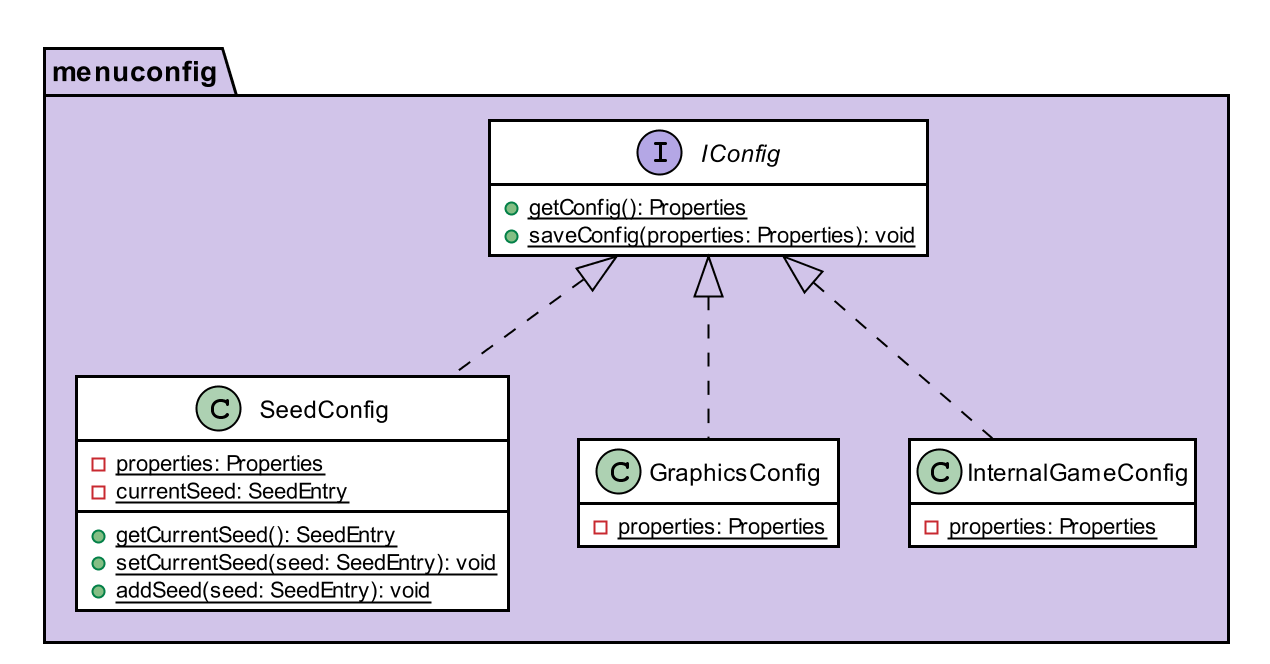
\includegraphics[width=\linewidth]{./GUI/GUI_Bilder/Config.png}
              \caption{Paket menuconfig}
               \label{fig:Config}
    \end{figure}

        \paragraph{\underline{IConfig}}\label{configlabel} \mbox{}\\
            Dieses Interface stellt Funktionen bereit, um Dateien zu laden und zu speichern.
            Jede Klasse die dieses Interface implementiert, muss die beiden Funktionen 
            überschreiben.

            \textbf{Methoden}					
            \begin{itemize}
                \item \textit{+ {static} getConfig(): Properties}
                    \begin{leftbar}[0.9\linewidth]
                        Gibt das Properties Objekt der Konfiguration zurück.\\
                        \textbf{@return} Das aktuelle Properties Objekt.
                    \end{leftbar}
                \item \textit{+ {static} saveConfig(Properties properties): void}
                    \begin{leftbar}[0.9\linewidth]
                        Überschreibt das aktuelle Properties Objekt mit dem übergebenem.\\
                        \textbf{@param properties} Das zu speichernde Properties Objekt.
                    \end{leftbar}
            \end{itemize}
            \pagebreak
        \paragraph{\underline{SeedConfig}} \mbox{}\\
            Diese Klasse verwaltet die Konfiguration der Seeds, bzw. speichert alle 
            vorhandenen Seeds in einer Datei, oder ergänzt diese um einen Seed. 
            Außerdem speichert sie den aktuell ausgewählten Seed.
            Ebenfalls wird das Interface~\nameref{configlabel} implementiert, um die Konfigurations Datei
            laden und speichern zu können. \par 
            \textbf{Attribute}
            \begin{itemize}
                \item \textit{- {static} Properties properties}
                    \begin{leftbar}[0.9\linewidth]
                        In diesem Properties Objekt werden die Einstellungen bzw Daten 
                        gespeichert.
                    \end{leftbar}
                \item \textit{- {static} currentSeedEntry: SeedEntry} 
                    \begin{leftbar}[0.9\linewidth]
                        Enthält den aktuell ausgewählten Seed.
                    \end{leftbar}
            \end{itemize}
            
            \textbf{Methoden}					
            \begin{itemize}
                \item \textit{+ {static} getCurrentSeed(): SeedEntry}
                    \begin{leftbar}[0.9\linewidth]
                        Gibt den aktuell ausgewählten Seed zurück.\\
                        \textbf{@return} Der aktuell ausgewählte Seed.
                    \end{leftbar}
                \item \textit{+ {static} setCurrentSeed(SeedEntry seed): void}
                    \begin{leftbar}[0.9\linewidth]
                        Überschreibt den aktuellen Seed mit einem neuen Seed Objekt.\\
                        \textbf{@param seed} Der zu speichernde Seed.
                    \end{leftbar}
                \item \textit{+ {static} addSeed(SeedEntry seed): void}
                    \begin{leftbar}[0.9\linewidth]
                        Fügt der SeedConfig Datei einen neuen Seed hinzu, wobei die 
                        Alten beibehalten werden.\\
                        \textbf{@param seed} Der Seed welcher hinzugefügt werden soll.
                    \end{leftbar}
            \end{itemize}

        \pagebreak
        \paragraph{\underline{GraphicsConfig}} \mbox{}\\
            Diese Klasse verwaltet die Konfiguration der im Menü einstellbaren 
            Grafikeinstellungen, bzw. speichert alle vorgenommen Änderungen der
            Grafik in einer Datei. 
            Ebenfalls wird das Interface~\nameref{configlabel} implementiert, um die Konfigurations Datei
            laden und speichern zu können. \par    
                    
            \textbf{Attribute}
            \begin{itemize}
                \item \textit{- {static} Properties properties}
                    \begin{leftbar}[0.9\linewidth]
                        In diesem Properties Objekt werden die Einstellungen bzw Daten 
                        gespeichert.
                    \end{leftbar}
            \end{itemize}
            
            \textbf{Methoden}					
            \begin{itemize}
                \item \textit{+ {static} getGraphicsConfig(): Properties}
                    \begin{leftbar}[0.9\linewidth]
                        Gibt das Properties Objekt der Grafik Konfiguration zurück.\\
                        \textbf{@return} Das aktuelle Properties Objekt.
                    \end{leftbar}
            \end{itemize}
		
		\paragraph{\underline{InternalGameConfig}} \mbox{}\\
            Diese Klasse verwaltet die Konfiguration der im Menü einstellbaren 
            internen Spieleinstellungen, bzw. speichert alle vorgenommen Änderungen
            in einer Datei. 
            Ebenfalls wird das Interface~\nameref{configlabel} implementiert, um die Konfigurations Datei
            laden und speichern zu können. \par    
                    
            \textbf{Attribute}
            \begin{itemize}
                \item \textit{- {static} Properties properties}
                    \begin{leftbar}[0.9\linewidth]
                        In diesem Properties Objekt werden die Einstellungen bzw Daten 
                        gespeichert.
                    \end{leftbar}
            \end{itemize}

    \pagebreak

\subsubsection{gui}\label{guipaket}
    Das gui Packet beinhaltet die Steuerungsklassen für alle grafischen
    Benutzeroberflächen des Spieles. Für jedes Menü existiert eine eigene
    Steuerungsklasse.
    Um Kontrolle über die Spieleapplikation zu haben existiert eine AppState Klasse, 
    welche von  \textit{com.jme3.app.state.AbstractAppState} erbt. Dies beinhaltet 
    die Bereitstellung der Information, ob und wenn ja,was für ein Menü-Bildschirm 
    geöffnet ist. Von dieser AppState Klasse erben weiterhin alle Steuerungsklassen, 
    die Zugriff auf die Applikation benötigen.
    Um auf Benuztereingaben und -aktionen reagieren zu können, wird ein
    Eingabe Mapping implementiert. \par

    \begin{center}
        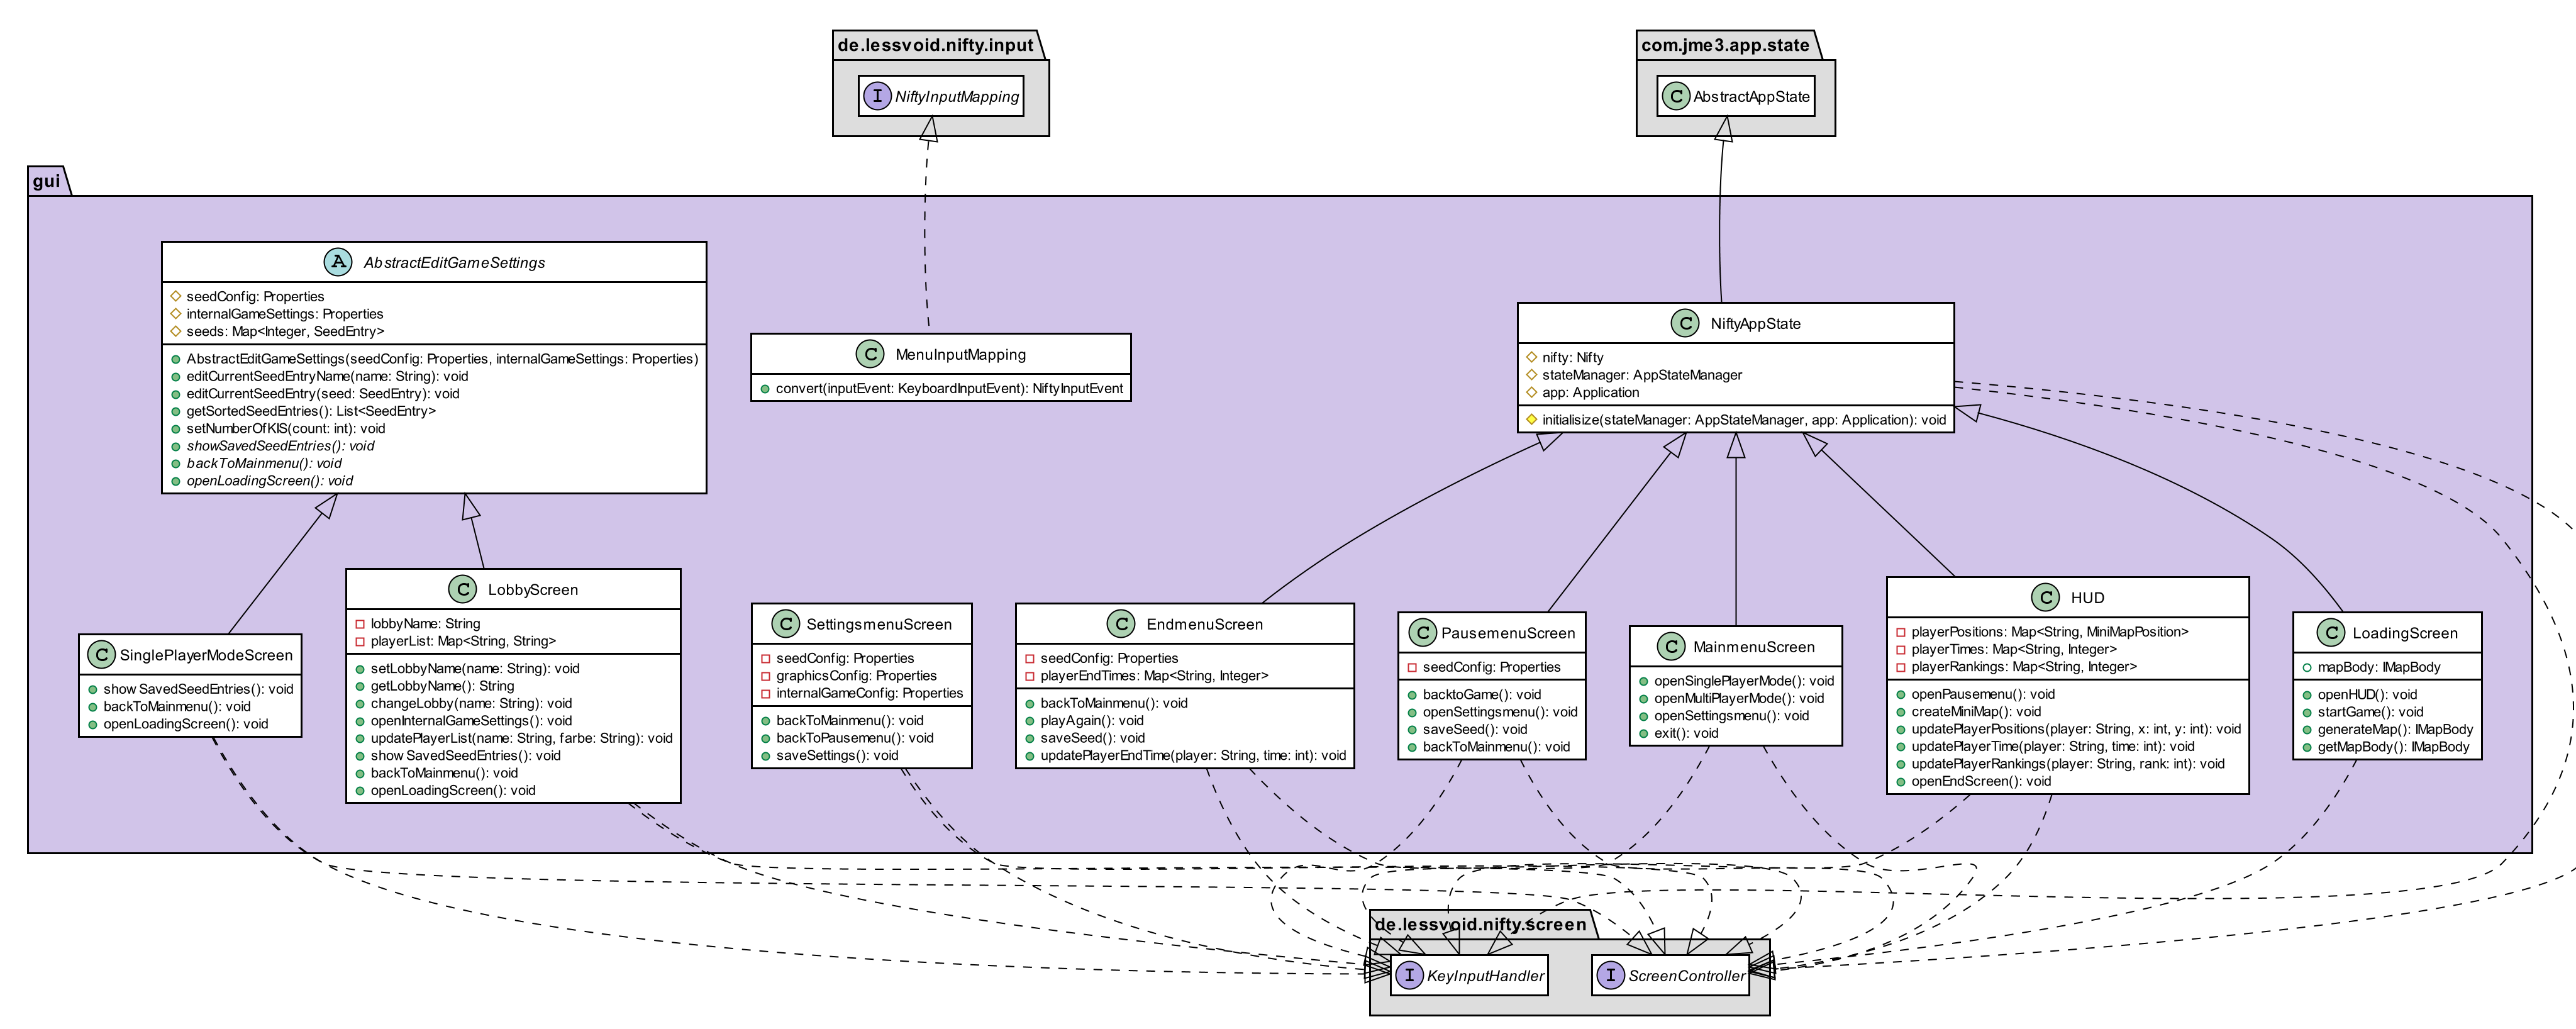
\includegraphics[width=0.85\linewidth]{./GUI/GUI_Bilder/GUI.png}
        \captionof{figure}{Paket gui}
        \label{fig:gui}
    \end{center}

        \pagebreak
        \paragraph{\underline{NiftyAppState}}\label{nas} \mbox{}\\
            Diese Klasse dient als Oberklasse für die meisten Steuerungsklassen 
            der grafischen Benutzeroberfläche des Spieles. Sie erbt von 
            \textit{com.jme3.app.state.AbstractAppState}, um Kontrolle über die 
            Spieleapplikation zu haben. Dies beinhaltet  die Bereitstellung der
            Information, ob und wenn ja, was für ein Menü-Bildschirm geöffnet ist. 
            Dazu wird zu gegebenem Anlass der jeweilige Menü-Bildschirm vom/an den
            StateManager entfernt/hinzugefügt.\\
            Um die Bildschirme steuern zu können, wird das Interface
            \textit{de.lessvoid.nifty.screen.ScreenController} implementiert und um auf
            Benuztereingaben und -aktionen reagieren zu können das Interface
            \textit{de.lessvoid.nifty.screen.KeyInputHandler}. Hierzu wird,
            auf die in der Klasse \textit{MenuInputMapping} bereits konvertierten
            Eingaben in NiftyInputEvents, entsprechend reagiert.\\ \par
            \textbf{Attribute}
            \begin{itemize}
                \item  \textit{\# Nifty nifty}
                    \begin{leftbar}[0.9\linewidth]
                        Referenz auf das Nifty Objekt.
                    \end{leftbar}
                \item  \textit{\# AppStateManager stateManager}  
                    \begin{leftbar}[0.9\linewidth]
                        Referenz auf den AppStateManager der Applikation.
                    \end{leftbar}
                \item  \textit{\# Application app} 
                    \begin{leftbar}[0.9\linewidth]
                        Referenz auf die Applikation.
                    \end{leftbar}
            \end{itemize}
            \textbf{Methoden}					
            \begin{itemize}
                \item  \textit{\# initialisize(AppStateManager stateManager, Application app): void} 
                    \begin{leftbar}[0.9\linewidth]
                        Initialisiert die Attribute und ruft explizit den Konstruktor
                        von AbstractAppState auf. \\
                        \textbf{@param stateManager} Der StateManager, welcher verwendet werden
                        soll.\\
                        \textbf{@param app} Die Applikation, welche verwendet werden
                        soll.\\
                    \end{leftbar}
            \end{itemize}

        \pagebreak
        \paragraph{\underline{MenuInputMapping}}\label{mim} \mbox{}\\
            Diese Klasse ist zuständig für die Konvertierung von Benuztereingaben
            und -aktionen in NiftyInputEvents. Sie ersetzt damit die von Nifty automatisch
            bereitgestellte MenuInputMapping Klasse.\\
            Um dies zu erreichen, wird das Interface 
            \textit{de.lessvoid.nifty.input.NiftyInputMapping} implementiert.
            Da die Steuerungsklassen nur von NiftyInputEvents abhängen, kann so mit wenigem
            Aufwand andere Geräte wie GamePads integriert werden. Dazu muss nur das Mapping
            erweitert werden.
            \par
                    
            \textbf{Methoden}					
            \begin{itemize}
                \item  \textit{+ convert(KeyboardInputEvent inputEvent): NiftyInputEvent} 
                    \begin{leftbar}[0.9\linewidth]
                        Erhält ein KeyboardInputEvent und konvertiert es in ein
                        NiftyInputEvent. Dieses NiftyInputEvent wird dann weiter 
                        geleitet an die Steuerungsklassen der grafischen 
                        Benutzeroberflächen. Die Escape, Enter und Pfeil-Tasten 
                        werden hier gemappt.\\
                        \textbf{@param inputEvent} Die Taste, welche auf der Tastatur
                        gedrückt wird.\\
                        \textbf{@return} Das gemappte NiftyInputEvent.
                    \end{leftbar}
            \end{itemize}
        
        \paragraph{\underline{AbstractEditGameSettings}}\label{adgs} \mbox{}\\
            Diese Klasse dient als Oberklasse für die Steuerungsklassen des
            Einzelspielermodus und Lobby Bildschirmes. Es enthält zwei abstrakte 
            Methoden, die von den erbenden Klassen implementiert werden müssen.
            In dieser Klasse werden interne Spieleeinstellungen vorgenommen, 
            wie Einstellung der Anzahl an KI's. Außerdem kann man 
            Seeds ändern und hinzufügen. \par
            
            \textbf{Attribute}
            \begin{itemize}
                \item \textit{\# Properties seedConfig}  
                    \begin{leftbar}[0.9\linewidth]
                        Referenz auf das Properties Objekt der Seed Konfiguration.
                    \end{leftbar}
                \item  \textit{\# Properties internalGameSettings} 
                    \begin{leftbar}[0.9\linewidth]
                        Referenz auf das Properties Objekt der internen 
                        Spieleeinstellungen.
                    \end{leftbar}
                \item  \textit{\# Map<Integer, SeedEntry> seeds} 
                    \begin{leftbar}[0.9\linewidth]
                        HashMap die alle gespeicherten Seeds des Spieles 
                        enthält. Dabei wird die Integer Zahlrenreihenfolge
                        des Seeds als Key gespeichert, damit dieser Unique
                        bleibt.
                    \end{leftbar}
            \end{itemize}
               
            \textbf{Methoden}					
            \begin{itemize}
                \item  \textit{+ AbstractEditGameSettings(Properties seedConfig, Properties internalGameSettings)} 
                    \begin{leftbar}[0.9\linewidth]
                        Konstruktor der die Attribute der Klasse initalisiert mit den
                        übergenen Parametern und die Map als HashMap initalisiert.\\
                        \textbf{@param seedConfig} Properties Objekt der Seed 
                        Konfiguration.\\
                        \textbf{@param internalGameSettings} Properties Objekt der 
                        internen Spieleeinstellungen.
                    \end{leftbar}
                \pagebreak
                \item  \textit{+ editCurrentSeedEntryName(String name): void} 
                    \begin{leftbar}[0.9\linewidth]
                        Überschreibt den Namen des aktuell ausgewählten
                        Seeds mit dem übergebenem String.\\
                        \textbf{@param name} Der zu speichernde String.\\
                    \end{leftbar}
                \item  \textit{+ editCurrentSeedEntry(SeedEntry seed): void} 
                    \begin{leftbar}[0.9\linewidth]
                        Überschreibt den aktuell ausgewählten Seed mit dem
                        übergebenem Seed.\\
                        \textbf{@param seed} Der zu speichernde Seed.\\
                    \end{leftbar}
                \item  \textit{+ getSortedSeedEntries(): List<SeedEntry>}
                    \begin{leftbar}[0.9\linewidth]
                        Gibt eine nach Namen sortierte SeedEntry Liste zurück.\\
                        \textbf{@return} Die sortierte SeedEntry Liste.
                    \end{leftbar}
                \item  \textit{+ setNumberOfKIS(int count): void} 
                    \begin{leftbar}[0.9\linewidth]
                        Setzt die Anzahl der KI's entsprechend der noch verfügbaren 
                        Plätze. Wenn 10 Spieler das Spiel spielen möchten, so kann 
                        keine KI hinzugefügt werden.\\
                        \textbf{@param count} Die zu setzende Anzahl an KI's.\\
                    \end{leftbar}
                \item  \textit{+ {abstract} showSavedSeeds(): void} 
                    \begin{leftbar}[0.9\linewidth]
                        Füllt das im Fenster anzuzeigende DropDown Menü mit den im Spiel
                        gespeicherten Seeds. Dazu wird die Methode \textit{getSortedSeedEntries()} aus
                        der selben Klasse aufgerufen. \\
                    \end{leftbar}
                \item  \textit{+ {abstract} backToMainmenu(): void} 
                    \begin{leftbar}[0.9\linewidth]
                        Kehrt aus dem aktuellen Fenster zum Hauptmenü zurück.\\
                    \end{leftbar}
                \item  \textit{+ {abstract} openLoadingScreen(): void} 
                    \begin{leftbar}[0.9\linewidth]
                        Geht aus dem aktuellen Fenster zum Lade Bildschirm.\\
                    \end{leftbar}
            \end{itemize}
        
        \pagebreak
		\paragraph{\underline{SinglePlayerModeScreen}} \mbox{}\\
            Diese Klasse dient der Steuerung der grafischen Benutzeroberfläche
            des Einzelmodus Bildschirmes. Sie setzt alle Klicks und Eingaben
            um und führt sie aus. Dazu erbt sie von~\nameref{adgs}, denn dort
            sind passende Methoden bereits implementiert und aufgelistet.\\
            Um die Bildschirme steuern zu können, wird das Interface
            \textit{de.lessvoid.nifty.screen.ScreenController} implementiert und um auf
            Benuztereingaben und -aktionen reagieren zu können das Interface
            \textit{de.lessvoid.nifty.screen.KeyInputHandler}.  \par

            \textbf{Methoden}					
            \begin{itemize}
                \item  \textit{+ showSavedSeeds(): void} 
                    \begin{leftbar}[0.9\linewidth]
                        Füllt das im Fenster anzuzeigende DropDown Menü mit den im Spiel
                        gespeicherten Seeds. Dazu wird die Methode \textit{getSortedSeedEntries()} aus
                        der geerbten Klasse aufgerufen. \\
                    \end{leftbar}
                \item  \textit{+ backToMainmenu(): void} 
                    \begin{leftbar}[0.9\linewidth]
                        Kehrt aus dem aktuellen Fenster zum Hauptmenü zurück.\\
                    \end{leftbar}
                \item  \textit{+ openLoadingScreen(): void} 
                    \begin{leftbar}[0.9\linewidth]
                        Geht aus dem aktuellen Fenster zum Lade Bildschirm.\\
                    \end{leftbar}
            \end{itemize}        
        
        \paragraph{\underline{LobbyScreen}} \mbox{}\\
            Diese Klasse dient der Steuerung der grafischen Benutzeroberfläche
            des Lobby Bildschirmes. Sie setzt alle Klicks und Eingaben
            um und führt sie aus. Dazu erbt sie von~\nameref{adgs}, denn dort
            sind passende Methoden bereits implementiert und aufgelistet.\\
            Um die Bildschirme steuern zu können, wird das Interface
            \textit{de.lessvoid.nifty.screen.ScreenController} implementiert und um auf
            Benuztereingaben und -aktionen reagieren zu können das Interface
            \textit{de.lessvoid.nifty.screen.KeyInputHandler}. \par
            
            \textbf{Attribute}
            \begin{itemize}
                \item \textit{- String lobbyName}  
                    \begin{leftbar}[0.9\linewidth]
                        Speichert den Namen der Lobby in der sich der Spieler 
                        aktuell befindet.\\
                    \end{leftbar}
                \item  \textit{- Map<String, String> playerList} 
                    \begin{leftbar}[0.9\linewidth]
                        Speichert alle Spieler, die der Lobby beigetreten sind 
                        sowie deren Farben als Hashmap.
                    \end{leftbar}
            \end{itemize}
               
            \textbf{Methoden}					
            \begin{itemize}
                \item  \textit{+ setLobbyName(String name): void} 
                    \begin{leftbar}[0.9\linewidth]
                        Überschreibt den Lobbynamen der aktuell 
                        beigetreten Lobby.\\
                        \textbf{@param name} Der zu speichernde Lobby Name.\\
                    \end{leftbar}
                \item  \textit{+ getLobbyName(): String} 
                    \begin{leftbar}[0.9\linewidth]
                        Gibt den Namen derjenigen Lobby zurück, in der 
                        sich der Spieler aktuell befindet.\\
                        \textbf{return} Der Lobby Name.\\
                    \end{leftbar}
                \item  \textit{+ changeLobby(String name): void} 
                    \begin{leftbar}[0.9\linewidth]
                        Wechselt die Lobby durch Eingabe eines anderen 
                        Lobby Namens. Existiert dieser nicht, kann 
                        auch nicht gewechselt werden.\\
                        \textbf{@param name} Der Namme der Lobby, zu der 
                        man wechseln möchte.\\
                    \end{leftbar}
                \item  \textit{+ openInternalGameSettings(): void} 
                    \begin{leftbar}[0.9\linewidth]
                        Öffnet ein Popup, in der die internen Spieleeinstellungen 
                        vorgenommen werden können.
                    \end{leftbar}
                \item  \textit{+ updatePlayerList(String name, String farbe): void} 
                    \begin{leftbar}[0.9\linewidth]
                        Sobald ein weiterer Spieler die Lobby betritt, 
                        aktualisiert sich die Hashmap.\\
                        \textbf{@param name} Der Name des neuen Spielers.\\
                        \textbf{@param farbe} Die Farbe des neuen Spielers, welche 
                        vom System selber gesetzt wird. Der Spieler hat darauf 
                        keinen Einfluss.\\
                    \end{leftbar}
                \item  \textit{+ showSavedSeeds(): void} 
                    \begin{leftbar}[0.9\linewidth]
                        Füllt das im Popup-Fenster anzuzeigende DropDown Menü mit den im Spiel
                        gespeicherten Seeds. Dazu wird die Methode \textit{getSortedSeedEntries()} aus
                        der geerbten Klasse aufgerufen. \\
                    \end{leftbar}
                \item  \textit{+ backToMainmenu(): void} 
                    \begin{leftbar}[0.9\linewidth]
                        Kehrt aus dem aktuellen Fenster zum Hauptmenü zurück.\\
                    \end{leftbar}
                \item  \textit{+ openLoadingScreen(): void} 
                    \begin{leftbar}[0.9\linewidth]
                        Geht aus dem aktuellen Fenster zum Lade Bildschrim.\\
                    \end{leftbar}
            \end{itemize}

        \pagebreak
        \paragraph{\underline{LoadingScreen}} \mbox{}\\
        Diese Klasse dient der Steuerung der grafischen Benutzeroberfläche
        des Lade Bildschirmes. Sie erbt von~\nameref{nas}, um Kontrolle über die 
        Spieleapplikation zu haben. Dies beinhaltet  die Bereitstellung der
        Information, ob und wenn ja, was für ein Menü-Bildschirm geöffnet ist.
        Dazu wird zu gegebenem Anlass der jeweilige Menü-Bildschirm vom/an den
        StateManager entfernt/hinzugefügt.\\
        Um die Bildschirme steuern zu können, wird das Interface
        \textit{de.lessvoid.nifty.screen.ScreenController} implementiert. \par
            
            \textbf{Attribute}
            \begin{itemize}
                \item \textit{+ IMapBody mapBody}  
                    \begin{leftbar}[0.9\linewidth]
                        Schnittstelle für das andere Team des PSE-Projektes.
                        Hier wird der Output des Strecken-Generatos gespeichert.
                    \end{leftbar}
            \end{itemize}
               
            \textbf{Methoden}					
            \begin{itemize}
                \item  \textit{+ openHUD(): void} 
                    \begin{leftbar}[0.9\linewidth]
                        Öffnet den Bildschirm des HUD's.\\
                    \end{leftbar}
                \item  \textit{+ startGame(): void} 
                    \begin{leftbar}[0.9\linewidth]
                        Hier werden alle AppStates, die während dem Rennen 
                        laufen sollen, initalisiert bzw an den AppStateManager
                        angehängt.
                    \end{leftbar}
                \item  \textit{+ generateMap(): IMapBody} 
                    \begin{leftbar}[0.9\linewidth]
                        Hier wird der Strecken-Generator aufgerufen, der dann 
                        einen Output liefert, welcher im Attribut mapBody 
                        gespeichert wird.
                    \end{leftbar}
                \item  \textit{+ getIMapBody(): IMapBody} 
                    \begin{leftbar}[0.9\linewidth]
                        Getter für das Attribut IMapBody.
                    \end{leftbar}
            \end{itemize}

		\paragraph{\underline{MainmenuScreen}} \mbox{}\\
            Diese Klasse dient der Steuerung der grafischen Benutzeroberfläche
            des Hauptmenü Bildschirmes. Sie erbt von~\nameref{nas}, um Kontrolle über die 
            Spieleapplikation zu haben. Dies beinhaltet  die Bereitstellung der
            Information, ob und wenn ja, was für ein Menü-Bildschirm geöffnet ist.
            Dazu wird zu gegebenem Anlass der jeweilige Menü-Bildschirm vom/an den
            StateManager entfernt/hinzugefügt.\\
            Um die Bildschirme steuern zu können, wird das Interface
            \textit{de.lessvoid.nifty.screen.ScreenController} implementiert und um auf
            Benuztereingaben und -aktionen reagieren zu können das Interface
            \textit{de.lessvoid.nifty.screen.KeyInputHandler}. \par
                        
            \textbf{Methoden}					
            \begin{itemize}
                \item  \textit{+ openSinglePlayerMode(): void} 
                    \begin{leftbar}[0.9\linewidth]
                        Wechselt zu dem Einzelspielermodus Bildschirm.\\
                    \end{leftbar}
                    \pagebreak
                \item  \textit{+ openMultiPlayerMode(): void} 
                    \begin{leftbar}[0.9\linewidth]
                        Wechselt zu dem Lobby Bildschirm.\\
                    \end{leftbar}
                \item  \textit{+ openSettingsmenu(): void} 
                    \begin{leftbar}[0.9\linewidth]
                        Wechselt zu dem Einstellungen Bildschirm.\\
                    \end{leftbar}
                \item  \textit{+ exit(): void} 
                    \begin{leftbar}[0.9\linewidth]
                        Beendet die Applikation.\\
                    \end{leftbar}
            \end{itemize}
        
        

        \paragraph{\underline{HUD}} \mbox{}\\
            Diese Klasse dient der Steuerung des HUD
            während des Rennens. Sie erbt von~\nameref{nas}, um Kontrolle über die 
            Spieleapplikation zu haben. Dies beinhaltet  die Bereitstellung der
            Information, ob und wenn ja, was für ein Menü-Bildschirm geöffnet ist.
            Dazu wird zu gegebenem Anlass der jeweilige Menü-Bildschirm vom/an den
            StateManager entfernt/hinzugefügt.\\
            Um die Bildschirme steuern zu können, wird das Interface
            \textit{de.lessvoid.nifty.screen.ScreenController} implementiert und um auf
            Benuztereingaben und -aktionen reagieren zu können das Interface
            \textit{de.lessvoid.nifty.screen.KeyInputHandler}. \par
            
            \textbf{Attribute}
            \begin{itemize}
                \item \textit{- Map<String, MiniMapPosition> playerPositions}  
                    \begin{leftbar}[0.9\linewidth]
                        Hashmap, welche zu jedem Spieler die aktuelle MiniMap-Position speichert.
                    \end{leftbar}
                \item  \textit{- Map<String, Integer> playerTimes} 
                    \begin{leftbar}[0.9\linewidth]
                        Hashmap, welche zu jedem Spieler seine bisher gefahrene Zeit enthält.
                    \end{leftbar}
                \item  \textit{- Map<String, Integer> playerRankings} 
                    \begin{leftbar}[0.9\linewidth]
                        Hashmap, welche zu jedem Spieler die Platzierung speichert.
                    \end{leftbar}
            \end{itemize}
               
            \textbf{Methoden}					
            \begin{itemize}
                \item  \textit{+ openPausemenu(): void} 
                    \begin{leftbar}[0.9\linewidth]
                        Öffnet das Pausemenü.\\
                    \end{leftbar}
                \item  \textit{+ createMiniMap(): void} 
                    \begin{leftbar}[0.9\linewidth]
                        Erstellt eine MiniMap, welche im HUD angezeigt werden soll.\\
                    \end{leftbar}
                    \pagebreak
                \item  \textit{+ updatePlayerPositions(String player, int x, int y): void} 
                    \begin{leftbar}[0.9\linewidth]
                        Aktualisiert die Position eines Spielers mit den gegebenen Koordinaten.\\
                        \textbf{@param player} Der Spieler, dessen Koordinaten aktualisiert
                        werden sollen.\\
                        \textbf{@param x} X-Koordinate des Spielers.\\
                        \textbf{@param y} Y-Koordinate des Spielers.\\
                    \end{leftbar}
                \item  \textit{+ updatePlayerTime(String player, int time): void} 
                    \begin{leftbar}[0.9\linewidth]
                        Aktualisiert die Zeit eines Spielers mit dem übergebenem Integer.\\
                        \textbf{@param player} Der Spieler, dessen zeit aktualisiert werden soll.\\
                        \textbf{@param time} Die neue Zeit des Spielers.\\
                    \end{leftbar}
                \item  \textit{+ updatePlayerRankings(String player, int rank): void} 
                    \begin{leftbar}[0.9\linewidth]
                        Aktualisiert die Platzierung des Spielers mit dem übergebenem Integer.\\
                        \textbf{@param player} Der Spieler, dessen Platzierung aktualisiert werden soll.\\
                        \textbf{@param rank} Die neue Platzierung des Spielers.\\
                    \end{leftbar}
                \item  \textit{+ openEndScreen(): void} 
                    \begin{leftbar}[0.9\linewidth]
                        Öffnet den Endmenü Bildschirm.\\
                    \end{leftbar}
            \end{itemize}

        \paragraph{\underline{PausemenuScreen}} \mbox{}\\
            Diese Klasse dient der Steuerung der grafischen Benutzeroberfläche
            des Pausemenü Bildschirmes. Sie erbt von~\nameref{nas}, um Kontrolle über die 
            Spieleapplikation zu haben. Dies beinhaltet  die Bereitstellung der
            Information, ob und wenn ja, was für ein Menü-Bildschirm geöffnet ist.
            Dazu wird zu gegebenem Anlass der jeweilige Menü-Bildschirm vom/an den
            StateManager entfernt/hinzugefügt.\\
            Um die Bildschirme steuern zu können, wird das Interface
            \textit{de.lessvoid.nifty.screen.ScreenController} implementiert und um auf
            Benuztereingaben und -aktionen reagieren zu können das Interface
            \textit{de.lessvoid.nifty.screen.KeyInputHandler}. \par
                
            \textbf{Attribute}
            \begin{itemize}
                \item \textit{- Properties seedConfig}  
                    \begin{leftbar}[0.9\linewidth]
                        Referenz auf das Properties Objekt der Seed Konfiguration.
                    \end{leftbar}
            \end{itemize}

            \textbf{Methoden}					
            \begin{itemize}
                \item  \textit{+ backtoGame(): void} 
                    \begin{leftbar}[0.9\linewidth]
                        Kehrt zum Spiel zurück.\\
                    \end{leftbar}
                \item  \textit{+ openSettingsmenu(): void} 
                    \begin{leftbar}[0.9\linewidth]
                        Öffnet das Einstellungsfenster.\\
                    \end{leftbar}
                \item  \textit{+ saveSeed(): void} 
                    \begin{leftbar}[0.9\linewidth]
                        Speichert einen Seed.\\
                    \end{leftbar}
                \item  \textit{+ backToMainmenu(): void} 
                    \begin{leftbar}[0.9\linewidth]
                        Kehrt zum Hauptmenü des Spieles zurück.\\
                    \end{leftbar}
            \end{itemize}

        
        \paragraph{\underline{SettingsmenuScreen}} \mbox{}\\
            Diese Klasse dient der Steuerung der grafischen Benutzeroberfläche
            des Einstellungs Bildschirmes. Sie erbt von~\nameref{nas}, um Kontrolle über die 
            Spieleapplikation zu haben. Dies beinhaltet  die Bereitstellung der
            Information, ob und wenn ja, was für ein Menü-Bildschirm geöffnet ist.
            Dazu wird zu gegebenem Anlass der jeweilige Menü-Bildschirm vom/an den
            StateManager entfernt/hinzugefügt.
            Um die Bildschirme steuern zu können, wird das Interface\\
            \textit{de.lessvoid.nifty.screen.ScreenController} implementiert und um auf
            Benuztereingaben und -aktionen reagieren zu können das Interface
            \textit{de.lessvoid.nifty.screen.KeyInputHandler}. \par
            
            \textbf{Attribute}
            \begin{itemize}
                \item \textit{- Properties seedConfig}  
                    \begin{leftbar}[0.9\linewidth]
                        Referenz auf das Properties Objekt der Seed Konfiguration.
                    \end{leftbar}
                \item  \textit{- Properties graphicsConfig} 
                    \begin{leftbar}[0.9\linewidth]
                        Referenz auf das Properties Objekt der Grafik Konfiguration.
                    \end{leftbar}
                \item  \textit{- Properties internalGameConfig} 
                    \begin{leftbar}[0.9\linewidth]
                        Referenz auf das Properties Objekt der internen Spiel Konfiguration.
                    \end{leftbar}
            \end{itemize}
               
            \textbf{Methoden}					
            \begin{itemize}
                \item  \textit{+ backToMainmenu(): void} 
                    \begin{leftbar}[0.9\linewidth]
                        Kehrt zum Hauptmenü zurück.\\
                    \end{leftbar}
                \item  \textit{+ backToPausemenu(): void} 
                    \begin{leftbar}[0.9\linewidth]
                        Kehrt zum Pausemenü zurück.\\
                    \end{leftbar}
                \item  \textit{+ saveSettings(): void} 
                    \begin{leftbar}[0.9\linewidth]
                        Speichert die Einstellungen.\\
                    \end{leftbar}
            \end{itemize}

        \pagebreak
        \paragraph{\underline{EndmenuScreen}} \mbox{}\\
        Diese Klasse dient der Steuerung der grafischen Benutzeroberfläche
        des Endmenü Bildschirmes. Sie erbt von~\nameref{nas}, um Kontrolle über die 
        Spieleapplikation zu haben. Dies beinhaltet  die Bereitstellung der
        Information, ob und wenn ja, was für ein Menü-Bildschirm geöffnet ist. \par
        Dazu wird zu gegebenem Anlass der jeweilige Menü-Bildschirm vom/an den
        StateManager entfernt/hinzugefügt.
        Um die Bildschirme steuern zu können, wird das Interface\\
        \textit{de.lessvoid.nifty.screen.ScreenController} implementiert und um auf
        Benuztereingaben und -aktionen reagieren zu können das Interface
        \textit{de.lessvoid.nifty.screen.KeyInputHandler}.\par
            
            \textbf{Attribute}
            \begin{itemize}
                \item \textit{- Properties seedConfig}  
                    \begin{leftbar}[0.9\linewidth]
                        Referenz auf das Properties Objekt der Seed Konfiguration.
                    \end{leftbar}
                \item  \textit{- Map<String, Integer> playerEndTimes} 
                    \begin{leftbar}[0.9\linewidth]
                        Hashmap, welche die endgültig gefahrenen Zeiten der Spieler enthält.
                    \end{leftbar}
            \end{itemize}
               
            \textbf{Methoden}					
            \begin{itemize}
                \item  \textit{+ backToMainmenu(): void} 
                    \begin{leftbar}[0.9\linewidth]
                        Kehrt zum Hauptmenü zurück.\\
                    \end{leftbar}
                \item  \textit{+ playAgain(): void} 
                    \begin{leftbar}[0.9\linewidth]
                        Ein erneutes Spiel wird gestartet, mit der selben Konfgiruation 
                        und Strecke.\\
                    \end{leftbar}
                \item  \textit{+ saveSeed(): void} 
                    \begin{leftbar}[0.9\linewidth]
                        Speichert den Seed.\\
                    \end{leftbar}
                \item  \textit{+ updatePlayerEndTime(String player, int time): void} 
                    \begin{leftbar}[0.9\linewidth]
                        Sobald ein Spieler ins Ziel gekommen ist, wird dieser dieser Hashmap 
                        hinzugefügt mit seiner gefahrenen Zeit.\\
                        \textbf{@param player} Der Spieler, welcher ins Ziel gekommen ist.\\
                        \textbf{@param time} Des Spielers gefahrene Zeit.\\
                    \end{leftbar}
            \end{itemize}
    \pagebreak